\documentclass[11pt]{article}
\usepackage[margin=1in]{geometry}
\usepackage{booktabs}
\usepackage{graphicx}
\usepackage{subcaption}
\usepackage{amsmath}
\usepackage{multirow}
\usepackage{float}
\usepackage{listings}
\usepackage{xcolor}
\usepackage{hyperref}

\graphicspath{{task1/plots/}}
\lstset{basicstyle=\ttfamily\small, columns=fullflexible, frame=single, breaklines=true}

\title{CS683 Programming Assignment II\\[4pt]
       \large Task 1: Stride Pattern Prefetching (SPP)}
\author{TEAM NAME \\ Member 1 (LDAP) \quad Member 2 (LDAP)}
\date{October 2026}

\begin{document}
\maketitle

\section*{Experimental Setup}
All simulations use ChampSim (single core, hashed-perceptron branch predictor, LRU
replacement at every level) with \textbf{25M warmup} and \textbf{25M simulation}
instructions on the three provided traces. Only the L1D prefetcher is changed
between configurations; every other cache level has no prefetcher.

\begin{itemize}
  \item \textbf{Baseline}: no prefetcher anywhere.
  \item \textbf{IP-stride}: the provided \texttt{prefetcher/ip\_stride.l1d\_pref} (degree 3).
  \item \textbf{SPP}: our \texttt{prefetcher/spp.l1d\_pref}.
\end{itemize}

Metrics are defined as in the assignment:
\[
\text{Speedup} = \frac{\text{IPC}_{\text{prefetcher}}}{\text{IPC}_{\text{baseline}}},\qquad
\text{Coverage} = \frac{\text{Misses}_{\text{baseline}} - \text{Misses}_{\text{prefetcher}}}{\text{Misses}_{\text{baseline}}},
\]
where \emph{Misses} are L1D load misses. L1D load MPKI and prefetch accuracy are
taken from ChampSim's statistics
(accuracy $=$ useful load prefetches $/$ prefetches issued to the lower level).
Raw outputs are in \texttt{results/}; tables and plots are produced by
\texttt{report/task1/parse\_task1.py}.

%=====================================================================
\section{Task 1A: IP-Stride Prefetcher}

The provided IP-stride prefetcher keeps a 24-entry fully associative tracker table
with LRU replacement, indexed by the low 8 bits of the load IP. Each entry stores the
last cache-line address accessed by that IP and the last observed stride.
On every L1D access:
\begin{enumerate}
  \item The IP is looked up. On a miss, the LRU entry is replaced and nothing is prefetched.
  \item The stride (current line $-$ last line) is computed. A stride of 0 is ignored.
  \item If the new stride equals the stored stride (the same stride seen twice in a row),
        it prefetches lines $A+s, A+2s, A+3s$ (degree 3), stopping at the 4\,KB page boundary.
        Prefetches fill into L1 when the MSHR is less than half full, otherwise into L2.
  \item The entry's last address and stride are updated.
\end{enumerate}
It only captures constant strides: any irregular but repeating sequence such as
$(+1,+2,+2,+2,+3)^n$ never produces two equal consecutive strides often enough to
trigger, which motivates SPP. Its results are included in the Task 1B tables as a reference point.

%=====================================================================
\section{Task 1B: Stride Pattern Prefetcher (SPP)}

\subsection{Design}

The design has two tables and a throttle:

\paragraph{IP table (64 entries, direct mapped).}
Indexed by \texttt{ip \% 64} with an 8-bit partial tag. Each entry tracks the last
line accessed by the IP, a \emph{uniform} stride with a 2-bit confidence counter, and a
9-bit \emph{signature} summarising the recent stride history.

\paragraph{Pattern table (512 entries, indexed by signature).}
Each entry maps a signature to the \emph{next expected stride} with a 2-bit confidence counter.
The signature is updated as
\[
\text{sig}_{\text{new}} = \big((\text{sig} \ll 3) \oplus (\text{stride} \,\&\, \texttt{0x3F})\big) \,\&\, \texttt{0x1FF},
\]
so it encodes roughly the last three strides. A repeating sequence such as
$(+1,+2,+2,+2,+3)^n$ produces a repeating series of signatures, and each one learns
which stride follows it.

\paragraph{Per-access operation.}
\begin{enumerate}
  \item \textbf{Lookup / allocate.} On a tag mismatch the entry is reset with the current
        line and no prefetch is issued.
  \item \textbf{Page change.} If the access is in a different 4\,KB page than the IP's
        last access, the history (stride, confidence, signature) is reset, because strides
        across pages are not meaningful in physical address space.
  \item \textbf{Uniform training.} If the stride matches the stored stride, confidence is
        incremented (saturating at 3), otherwise decremented. The stored stride is replaced
        only once confidence reaches 0 (hysteresis).
  \item \textbf{Non-uniform training.} The pattern-table entry for the current signature is
        trained with the observed stride in the same way, then the signature is updated.
  \item \textbf{Dual pattern classification and prefetch.}
    \begin{itemize}
      \item If uniform confidence $\geq 2$, the IP is classified as \textbf{uniform} and we
            prefetch $A+s, A+2s, \dots, A+\text{degree}\cdot s$.
      \item Otherwise it \textbf{falls back to non-uniform}: starting from the current
            signature, we walk the pattern table (lookahead), adding each predicted stride and
            updating a speculative signature, for up to \emph{degree} steps. The walk stops at
            any entry with confidence $<1$.
    \end{itemize}
    Uniform prediction therefore has priority. When a constant stride breaks, its confidence
    counter decays to below 2 within a couple of accesses and the IP automatically switches
    to signature-based prediction. The switch back happens when the constant stride is seen
    again.
  \item \textbf{Page boundary.} Every candidate prefetch is checked to be in the same page as
        the demand access, and the walk stops at the first one that would cross it.
        As in IP-stride, prefetches fill into L1 when MSHR occupancy is below half, otherwise into L2.
\end{enumerate}

\paragraph{Accuracy-based throttling.}
Accuracy is measured in epochs of 256 prefetches issued to the lower level. At the end of
each epoch,
$\text{acc} = \frac{\Delta\,\text{useful prefetches}}{\Delta\,\text{prefetches issued}}$
over that epoch, and the degree for the next epoch is set as:
\begin{center}
\begin{tabular}{cc}
\toprule
Epoch accuracy & Degree \\
\midrule
$\geq 75\%$ & 4 \\
$50$--$75\%$ & 3 \\
$25$--$50\%$ & 2 \\
$< 25\%$ & 1 \\
\bottomrule
\end{tabular}
\end{center}
The initial degree is 2. A counter reset at the end of warmup is detected and simply restarts the epoch.

%---------------------------------------------------------------------
\subsection{Results}

\begin{table}[H]
\centering
\caption{Task 1 results (25M warmup + 25M simulation instructions).}
\label{tab:main}
\begin{tabular}{llrrrrr}
\toprule
Trace & Config & IPC & Speedup & L1D Load MPKI & Accuracy (\%) & Coverage (\%) \\
\midrule
\multirow{3}{*}{Trace1} & Baseline  & 0.2322 & 1.0000 & 10.679 & --    & --    \\
                        & IP-stride & 0.2333 & 1.0047 & 10.118 & 52.97 & 5.25  \\
                        & SPP       & 0.2343 & \textbf{1.0089} & \textbf{9.642}  & \textbf{54.68} & \textbf{9.71}  \\
\midrule
\multirow{3}{*}{Trace2} & Baseline  & 0.2513 & 1.0000 & 13.536 & --    & --    \\
                        & IP-stride & 0.2512 & 0.9995 & 13.438 & 38.00 & 0.72  \\
                        & SPP       & 0.2531 & \textbf{1.0072} & \textbf{13.155} & \textbf{49.23} & \textbf{2.82}  \\
\midrule
\multirow{3}{*}{Trace3} & Baseline  & 0.3819 & 1.0000 & 3.403  & --    & --    \\
                        & IP-stride & 0.3827 & 1.0022 & 3.319  & 15.95 & 2.49  \\
                        & SPP       & 0.3888 & \textbf{1.0183} & \textbf{2.914}  & \textbf{45.82} & \textbf{14.39} \\
\midrule
\multirow{2}{*}{Mean$^\dagger$} & IP-stride & 0.2820 & 1.0021 & 8.958 & 35.64 & 2.82 \\
                                & SPP       & 0.2846 & \textbf{1.0114} & \textbf{8.570} & \textbf{49.91} & \textbf{8.97} \\
\bottomrule
\end{tabular}

\smallskip
{\footnotesize $^\dagger$Geometric mean for IPC and speedup; arithmetic mean for MPKI, accuracy and coverage.}
\end{table}

\begin{figure}[H]
\centering
\begin{subfigure}{0.49\textwidth}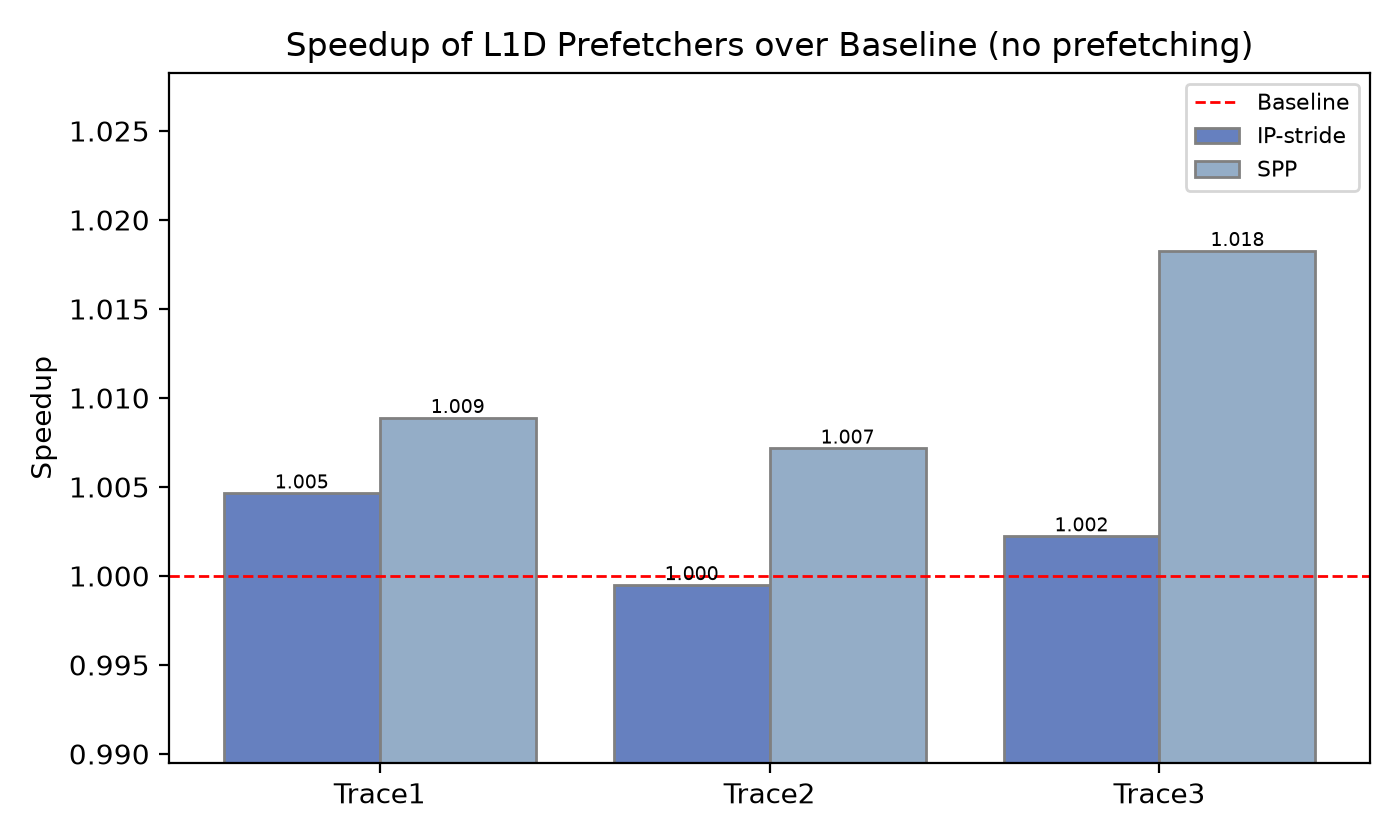
\includegraphics[width=\linewidth]{speedup.png}\caption{Speedup}\end{subfigure}
\begin{subfigure}{0.49\textwidth}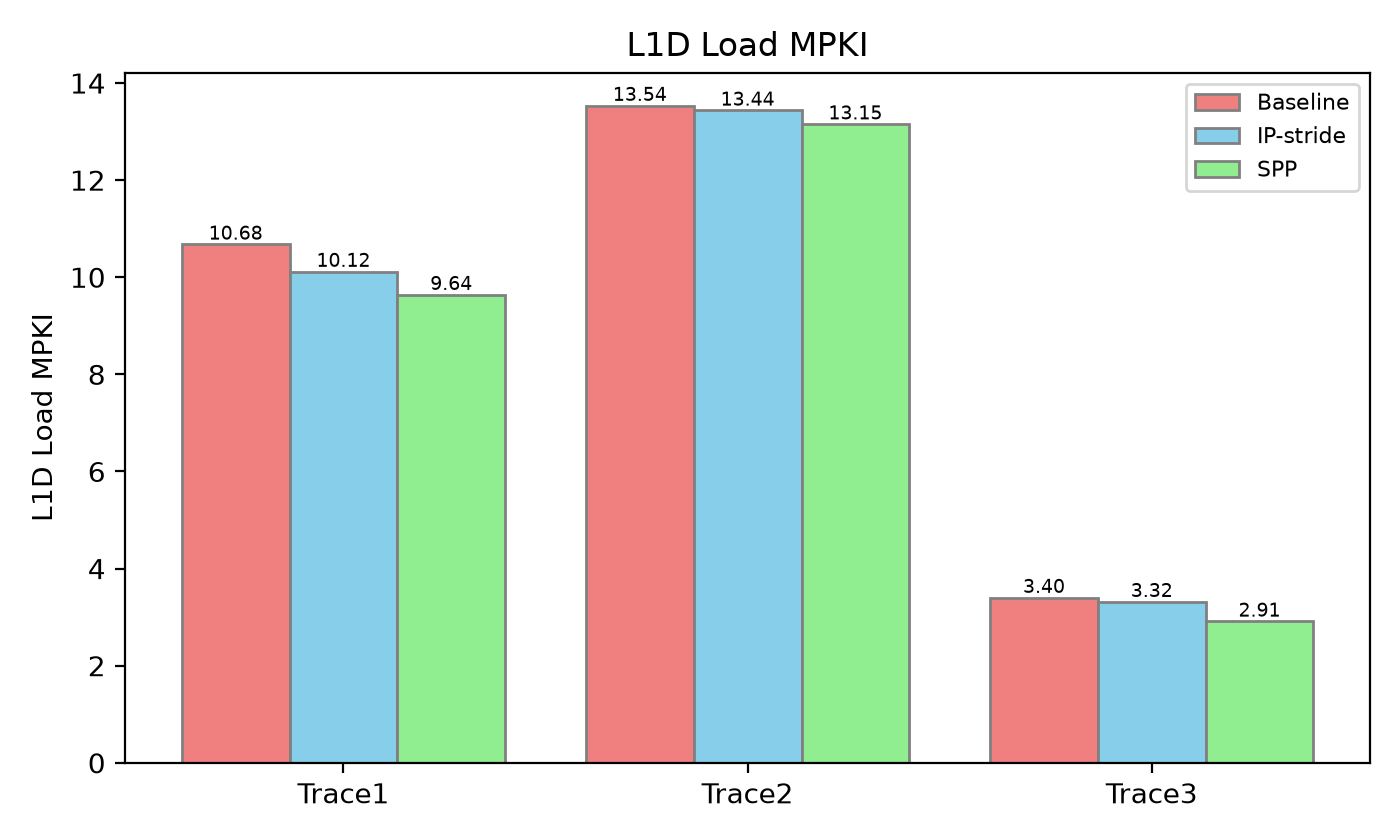
\includegraphics[width=\linewidth]{mpki.png}\caption{L1D load MPKI}\end{subfigure}\\[4pt]
\begin{subfigure}{0.49\textwidth}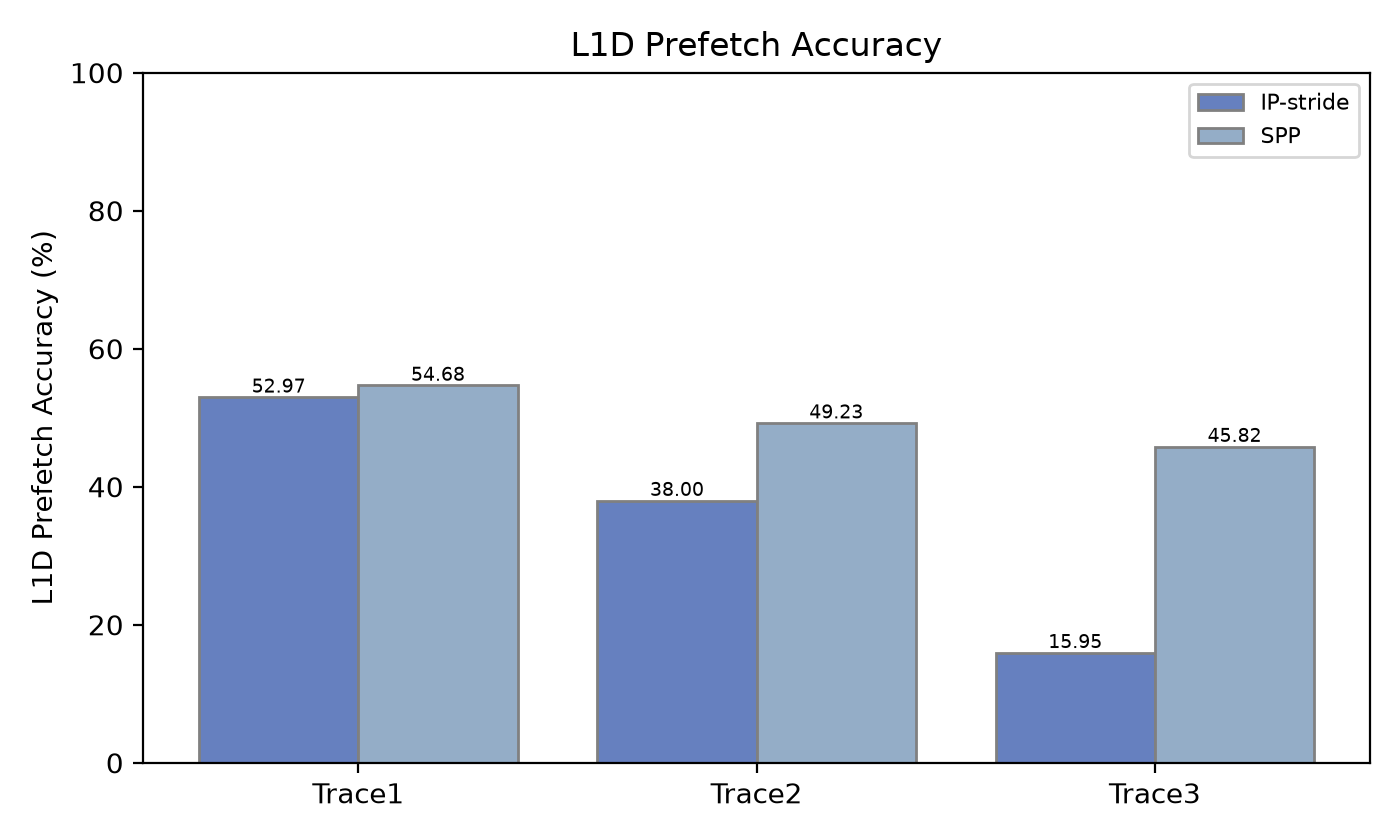
\includegraphics[width=\linewidth]{accuracy.png}\caption{Prefetch accuracy}\end{subfigure}
\begin{subfigure}{0.49\textwidth}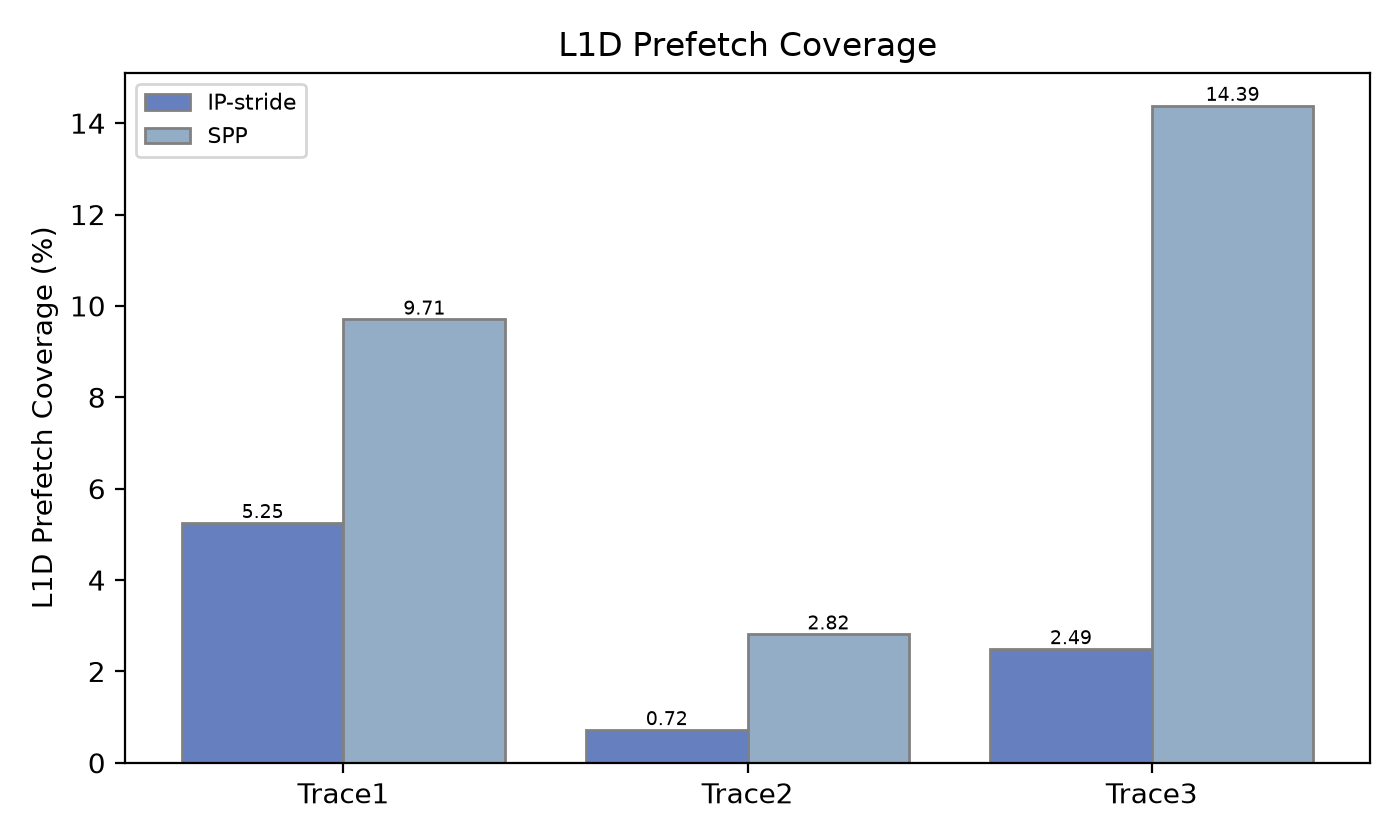
\includegraphics[width=\linewidth]{coverage.png}\caption{Prefetch coverage}\end{subfigure}
\caption{IP-stride vs.\ SPP at the L1D.}
\label{fig:main}
\end{figure}

\begin{figure}[H]
\centering
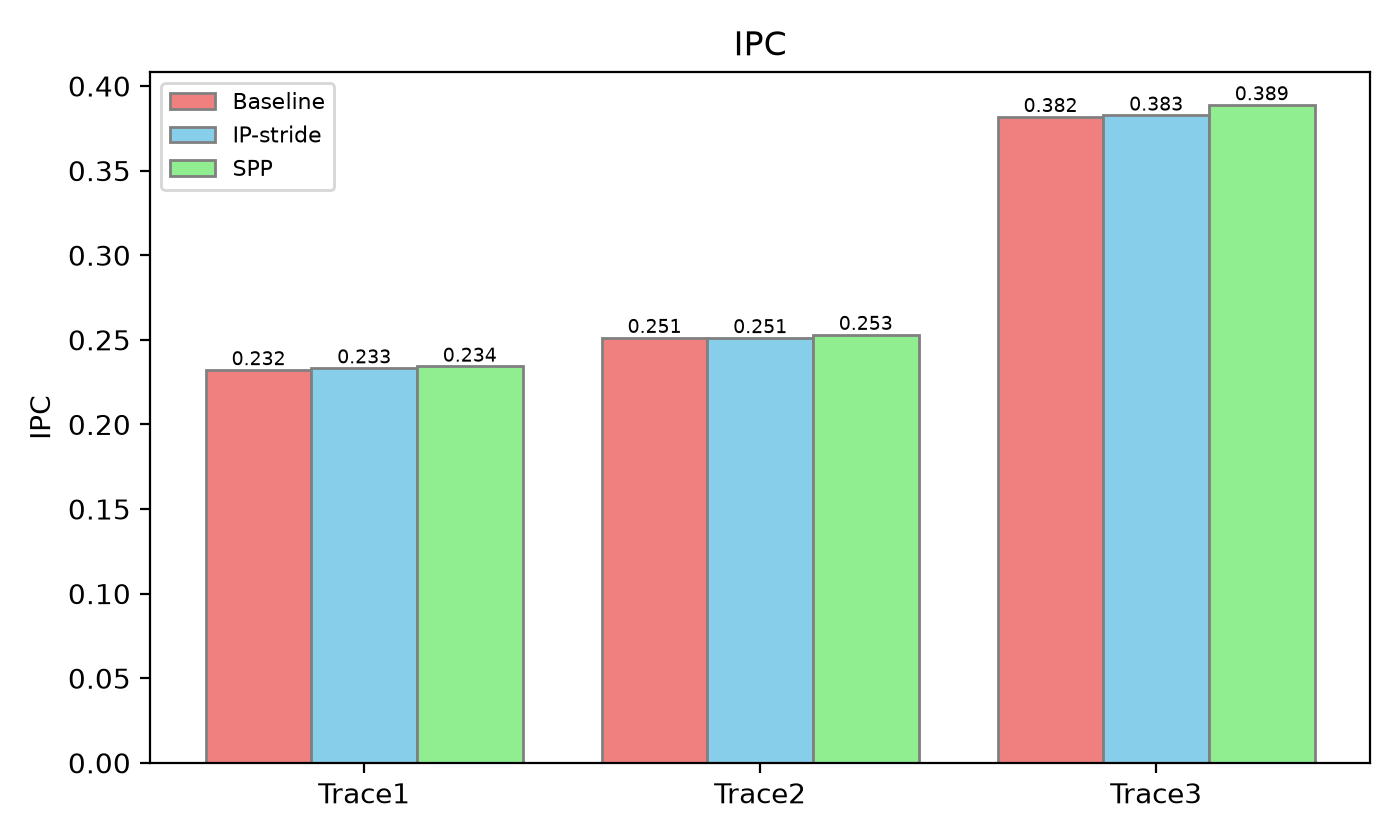
\includegraphics[width=0.6\linewidth]{ipc.png}
\caption{IPC of Baseline, IP-stride and SPP.}
\end{figure}

\paragraph{Observations.}
\begin{itemize}
  \item SPP outperforms IP-stride on every trace in all four metrics. Its geomean speedup is
        1.0114 vs.\ 1.0021 for IP-stride, and it lowers average L1D load MPKI from 9.21
        (baseline) to 8.57, vs.\ 8.96 for IP-stride.
  \item On \textbf{Trace3} SPP reaches 14.4\% coverage vs.\ 2.5\% for IP-stride, and
        accuracy rises from 16\% to 46\%. This large gap suggests that the stream contains
        irregular but repeating stride sequences, which IP-stride cannot capture (it prefetches
        wrongly when two strides coincidentally match) but the signature table can.
  \item On \textbf{Trace2} IP-stride is slightly \emph{slower} than the baseline (0.9995).
        Its fixed degree 3 at 38\% accuracy pollutes the L1D. SPP stays at 49\% accuracy,
        because its throttle keeps the degree low when accuracy is below 50\%, and gains 0.72\%.
  \item Absolute speedups are small because all three traces are memory-bound
        (IPC $\approx$ 0.23--0.38) and coverage stays modest (3--14\%). Most L1D
        misses are not predictable within a 4\,KB page by an IP-local prefetcher.
\end{itemize}

%---------------------------------------------------------------------
\subsection{Storage Overhead}

Field widths are the minimum needed by the logic. Strides are in cache lines and never cross
a 4\,KB page (64 lines), so they lie in $[-63,+63]$ and need 7 bits (signed).

\begin{table}[H]
\centering
\caption{IP table entry (64 entries).}
\begin{tabular}{lrl}
\toprule
Field & Bits & Purpose \\
\midrule
\texttt{valid}     & 1  & entry in use \\
\texttt{tag}       & 8  & partial IP tag, \texttt{(ip / 64) \& 0xFF} \\
\texttt{last\_line}& 58 & last line address (64-bit address $-$ 6 block-offset bits) \\
\texttt{stride}    & 7  & uniform stride, $[-63,+63]$ \\
\texttt{conf}      & 2  & uniform confidence, 0--3 \\
\texttt{sig}       & 9  & stride-history signature \\
\midrule
\textbf{Total per entry} & \textbf{85} & \\
\textbf{Table total} & \multicolumn{2}{l}{$64 \times 85 = \mathbf{5440}$ bits} \\
\bottomrule
\end{tabular}
\end{table}

\begin{table}[H]
\centering
\caption{Pattern table entry (512 entries, indexed by the 9-bit signature, so no tag).}
\begin{tabular}{lrl}
\toprule
Field & Bits & Purpose \\
\midrule
\texttt{next} & 7 & predicted next stride, $[-63,+63]$ \\
\texttt{conf} & 2 & confidence, 0--3 \\
\midrule
\textbf{Total per entry} & \textbf{9} & \\
\textbf{Table total} & \multicolumn{2}{l}{$512 \times 9 = \mathbf{4608}$ bits} \\
\bottomrule
\end{tabular}
\end{table}

\begin{table}[H]
\centering
\caption{Throttling state (global).}
\begin{tabular}{lrl}
\toprule
Field & Bits & Purpose \\
\midrule
\texttt{degree}            & 2 & current degree 1--4 (stored as degree$-1$) \\
epoch prefetch counter     & 9 & prefetches issued in this epoch (up to 256, plus overshoot) \\
epoch useful counter       & 9 & useful prefetches in this epoch \\
\midrule
\textbf{Total} & \textbf{20} & \\
\bottomrule
\end{tabular}
\end{table}

In the simulator the throttle stores 64-bit snapshots of ChampSim's global counters for
convenience. In hardware, two 9-bit counters reset at each epoch are equivalent.

\[
\text{Total} = 5440 + 4608 + 20 = \mathbf{10068\ bits} \approx \mathbf{1258.5\ bytes} \;(\approx 1.23\ \text{KB}).
\]

The largest field is \texttt{last\_line} (58 bits). It could be reduced to a 6-bit page
offset plus a hashed page tag of about 16 bits, bringing the IP table to 2240 bits, but we report
the design exactly as implemented.

%---------------------------------------------------------------------
\subsection{Choice of Accuracy Thresholds and Degrees}

\paragraph{How the thresholds were decided.}
The goal of throttling is to use a large degree only when extra prefetches are likely to be
useful. Accuracy is a fraction in $[0,100]\%$ and we have four degree levels, so we started
from an even quartile split (75/50/25). We then ran a sensitivity study comparing it
against (i) fixed degrees 1--4 with throttling disabled, (ii) a conservative split
90/70/50 and (iii) an aggressive split 60/40/20. All other parameters were kept unchanged.

\begin{table}[H]
\centering
\caption{Sensitivity of SPP to degree and throttling thresholds (speedup / accuracy\% / coverage\%).}
\label{tab:sens}
\small
\begin{tabular}{lccccc}
\toprule
Config & Trace1 & Trace2 & Trace3 & Geomean SU & Prefetches to L2$^\ddagger$ \\
\midrule
Fixed degree 1 & 1.0079 / 56.97 / 7.25  & 1.0049 / 48.84 / 1.97 & 1.0112 / 42.23 / 9.14  & 1.0080 & 79{,}161 \\
Fixed degree 2 & 1.0090 / 55.17 / 9.13  & 1.0062 / 46.48 / 2.54 & 1.0159 / 39.75 / 13.50 & 1.0103 & 114{,}840 \\
Fixed degree 3 & 1.0086 / 51.89 / 10.02 & 1.0062 / 42.41 / 2.67 & 1.0183 / 37.97 / 15.91 & 1.0110 & 140{,}639 \\
Fixed degree 4 & 1.0082 / 49.01 / 10.53 & 1.0063 / 38.57 / 2.67 & 1.0200 / 36.20 / 17.79 & 1.0115 & 164{,}024 \\
\midrule
Thr 90/70/50   & 1.0087 / 57.34 / 8.69  & 1.0069 / 52.69 / 2.65 & 1.0162 / 47.26 / 11.83 & 1.0106 & 95{,}566 \\
\textbf{Thr 75/50/25 (final)} & 1.0089 / 54.68 / 9.71 & 1.0072 / 49.23 / 2.82 & 1.0183 / 45.82 / 14.39 & \textbf{1.0114} & \textbf{116{,}834} \\
Thr 60/40/20   & 1.0090 / 53.42 / 10.03 & 1.0072 / 47.17 / 2.85 & 1.0191 / 45.81 / 15.33 & 1.0118 & 125{,}536 \\
\bottomrule
\end{tabular}

\smallskip
{\footnotesize $^\ddagger$Total prefetches issued to the lower level, summed over the three traces (a proxy for extra memory traffic).}
\end{table}

\begin{figure}[H]
\centering
\begin{subfigure}{0.49\textwidth}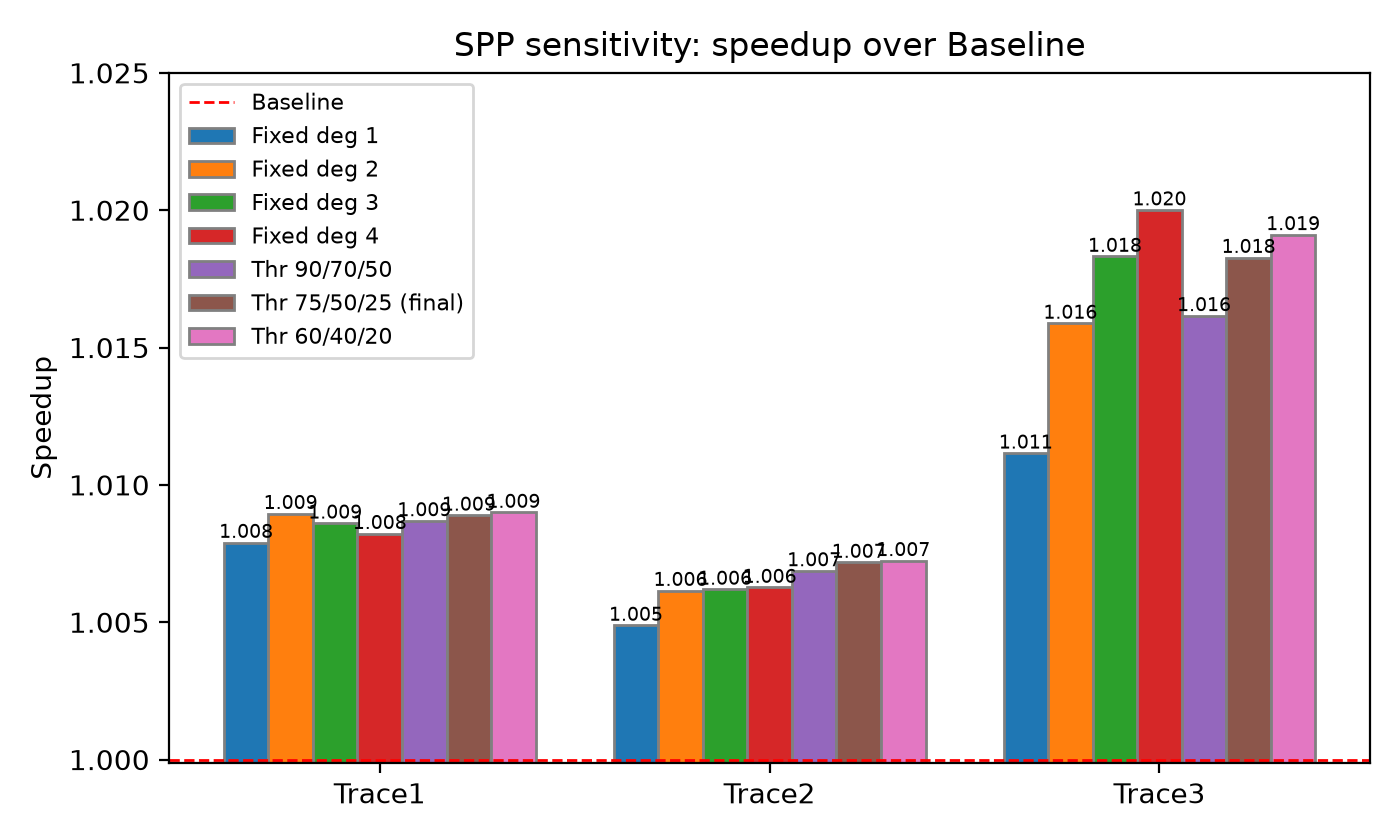
\includegraphics[width=\linewidth]{sens_speedup.png}\caption{Speedup}\end{subfigure}
\begin{subfigure}{0.49\textwidth}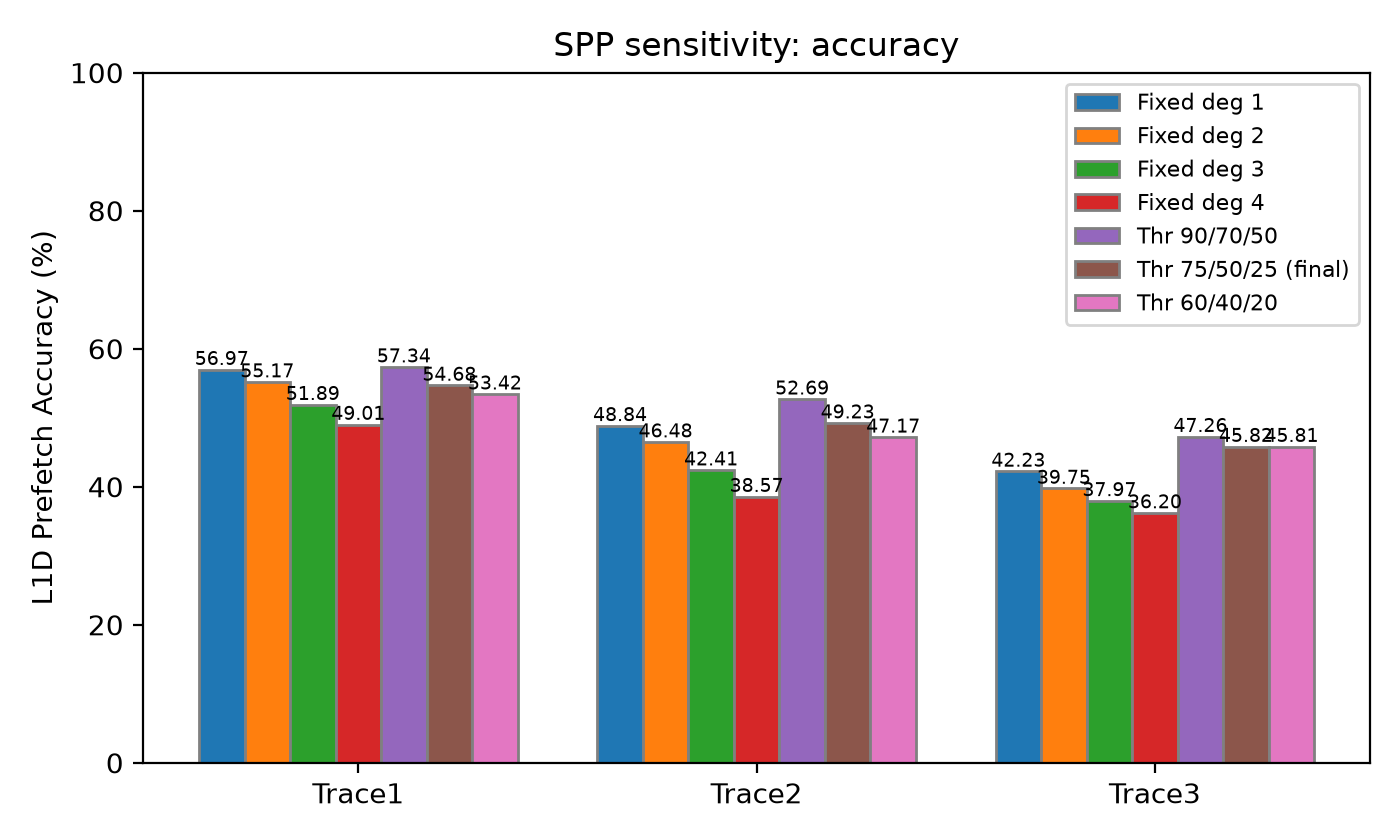
\includegraphics[width=\linewidth]{sens_accuracy.png}\caption{Accuracy}\end{subfigure}
\caption{Sensitivity study of SPP degree and thresholds.}
\end{figure}

\paragraph{What the study shows.}
\begin{itemize}
  \item \textbf{No single fixed degree is best everywhere.} Trace1 peaks at degree 2 and gets
        \emph{slower} at degrees 3 and 4. Trace3 keeps improving up to degree 4. Raising the
        degree always lowers accuracy (e.g.\ Trace2 drops from 48.8\% to 38.6\%) while coverage
        saturates (Trace2 coverage is flat beyond degree 3). This is exactly the case for
        accuracy-based throttling.
  \item \textbf{Throttling gives most of the benefit of a large degree at a lower cost.} The final
        75/50/25 setting reaches a geomean speedup of 1.0114, within 0.01\% of fixed degree 4
        (1.0115), but issues \textbf{29\% fewer} prefetches (116.8K vs.\ 164.0K) at 8.6 points
        higher average accuracy (49.9\% vs.\ 41.3\%). It is also within 0.03\% of the best
        result on Trace1 and Trace2.
  \item \textbf{Conservative thresholds (90/70/50)} have the best accuracy, but they rarely
        allow degree 3--4, so Trace3 loses coverage (11.8\% vs.\ 14.4\%) and speedup.
  \item \textbf{Aggressive thresholds (60/40/20)} are marginally faster (geomean 1.0118 vs.\ 1.0114)
        but issue 7.4\% more prefetches for that 0.04\% gain. Both their accuracy and their
        advantage shrink as more prefetches are sent.
\end{itemize}
We chose 75/50/25 as the balance point. It is essentially tied with the fastest
configurations while keeping accuracy close to 50\% and limiting cache pollution and memory
traffic. This matters in a full system where the L2/LLC and DRAM bandwidth are shared, and
it is the stated goal of the throttle.

\paragraph{Why these degrees for each accuracy range.}
The degree is chosen so that the \emph{expected number of useful prefetches per trigger}
grows with accuracy while the \emph{expected number of useless prefetches} stays bounded
at about 1--2:
\begin{itemize}
  \item \textbf{$\geq 75\%$ $\rightarrow$ degree 4.} At high accuracy, 4 prefetches yield about 3
        useful lines and at most 1 useless one. Lookahead also improves timeliness: deeper
        prefetches are issued earlier relative to their demand (Trace3 late prefetches
        drop from 5262 at degree 2 to 3970 at degree 4).
        We cap the degree at 4 because a deeper signature walk compounds prediction errors
        (each lookahead step multiplies the probabilities), and coverage was already
        saturating at degree 3--4 in the study.
  \item \textbf{$50$--$75\%$ $\rightarrow$ degree 3.} Each prefetch is still more likely to be useful
        than not, so lookahead is worth it, but one step less to limit wasted lines.
  \item \textbf{$25$--$50\%$ $\rightarrow$ degree 2.} Fewer than half the prefetches help. Degree 2
        still covers the immediate next access plus one lookahead, which helped all traces
        compared to degree 1 (fixed degree 2 beats fixed degree 1 on every trace).
  \item \textbf{$< 25\%$ $\rightarrow$ degree 1.} Most prefetches are wasted. We keep a minimum
        degree of 1 rather than disabling the prefetcher, so it keeps issuing (and measuring)
        prefetches and can recover when the program enters a more predictable phase.
        A degree of 0 would leave no useful-prefetch feedback to raise accuracy again.
\end{itemize}
The epoch length of 256 prefetches is long enough for a statistically stable accuracy
estimate (one useful prefetch changes it by only 0.4\%) yet short enough to react to
program phases within a few thousand accesses.

\end{document}
